%**************************************%
%* Generated from MathBook XML source *%
%*    on 2016-07-13T11:07:04-04:00    *%
%*                                    *%
%*   http://mathbook.pugetsound.edu   *%
%*                                    *%
%**************************************%
\documentclass[10pt,]{book}
%% Load geometry package to allow page margin adjustments
\usepackage{geometry}
\geometry{letterpaper,total={5.0in,9.0in}}
%% Custom Preamble Entries, early (use latex.preamble.early)
%% Inline math delimiters, \(, \), need to be robust
%% 2016-01-31:  latexrelease.sty  supersedes  fixltx2e.sty
%% If  latexrelease.sty  exists, bugfix is in kernel
%% If not, bugfix is in  fixltx2e.sty
%% See:  https://tug.org/TUGboat/tb36-3/tb114ltnews22.pdf
%% and read "Fewer fragile commands" in distribution's  latexchanges.pdf
\IfFileExists{latexrelease.sty}{}{\usepackage{fixltx2e}}
%% Page Layout Adjustments (latex.geometry)
%% For unicode character support, use the "xelatex" executable
%% If never using xelatex, the next three lines can be removed
\usepackage{ifxetex}
\ifxetex\usepackage{xltxtra}\fi
%% Symbols, align environment, bracket-matrix
\usepackage{amsmath}
\usepackage{amssymb}
%% allow more columns to a matrix
%% can make this even bigger by overriding with  latex.preamble.late  processing option
\setcounter{MaxMatrixCols}{30}
%% Semantic Macros
%% To preserve meaning in a LaTeX file
%% Only defined here if required in this document
%% Used for inline definitions of terms
\newcommand{\terminology}[1]{\textbf{#1}}
%% Used for fillin answer blank
%% Argument is length in em
\newcommand{\fillin}[1]{\rule{#1em}{0.1ex}}
%% Subdivision Numbering, Chapters, Sections, Subsections, etc
%% Subdivision numbers may be turned off at some level ("depth")
%% A section *always* has depth 1, contrary to us counting from the document root
%% The latex default is 3.  If a larger number is present here, then
%% removing this command may make some cross-references ambiguous
%% The precursor variable $numbering-maxlevel is checked for consistency in the common XSL file
\setcounter{secnumdepth}{1}
%% Environments with amsthm package
%% Theorem-like environments in "plain" style, with or without proof
\usepackage{amsthm}
\theoremstyle{plain}
%% Numbering for Theorems, Conjectures, Examples, Figures, etc
%% Controlled by  numbering.theorems.level  processing parameter
%% Always need a theorem environment to set base numbering scheme
%% even if document has no theorems (but has other environments)
\newtheorem{theorem}{Key Fact}[section]
%% Only variants actually used in document appear here
%% Style is like a theorem, and for statements without proofs
%% Numbering: all theorem-like numbered consecutively
%% i.e. Corollary 4.3 follows Theorem 4.2
%% Remark-like environments, normal text
%% Numbering is in sync with theorems, etc
\theoremstyle{definition}
\newtheorem{remark}[theorem]{Remark}
\newtheorem{warning}[theorem]{Caution}
%% Example-like environments, normal text
%% Numbering is in sync with theorems, etc
\theoremstyle{definition}
\newtheorem{example}[theorem]{Example}
%% Miscellaneous environments, normal text
%% Numbering for inline exercises and lists is in sync with theorems, etc
\theoremstyle{definition}
\newtheorem{exercise}[theorem]{Exercise}
%% Localize LaTeX supplied names (possibly none)
\renewcommand*{\chaptername}{Chapter}
%% For improved tables
\usepackage{array}
%% Some extra height on each row is desirable, especially with horizontal rules
%% Increment determined experimentally
\setlength{\extrarowheight}{0.2ex}
%% Define variable thickness horizontal rules, full and partial
%% Thicknesses are 0.03, 0.05, 0.08 in the  booktabs  package
\makeatletter
\newcommand{\hrulethin}  {\noalign{\hrule height 0.04em}}
\newcommand{\hrulemedium}{\noalign{\hrule height 0.07em}}
\newcommand{\hrulethick} {\noalign{\hrule height 0.11em}}
%% We preserve a copy of the \setlength package before other
%% packages (extpfeil) get a chance to load packages that redefine it
\let\oldsetlength\setlength
\newlength{\Oldarrayrulewidth}
\newcommand{\crulethin}[1]%
{\noalign{\global\oldsetlength{\Oldarrayrulewidth}{\arrayrulewidth}}%
\noalign{\global\oldsetlength{\arrayrulewidth}{0.04em}}\cline{#1}%
\noalign{\global\oldsetlength{\arrayrulewidth}{\Oldarrayrulewidth}}}%
\newcommand{\crulemedium}[1]%
{\noalign{\global\oldsetlength{\Oldarrayrulewidth}{\arrayrulewidth}}%
\noalign{\global\oldsetlength{\arrayrulewidth}{0.07em}}\cline{#1}%
\noalign{\global\oldsetlength{\arrayrulewidth}{\Oldarrayrulewidth}}}
\newcommand{\crulethick}[1]%
{\noalign{\global\oldsetlength{\Oldarrayrulewidth}{\arrayrulewidth}}%
\noalign{\global\oldsetlength{\arrayrulewidth}{0.11em}}\cline{#1}%
\noalign{\global\oldsetlength{\arrayrulewidth}{\Oldarrayrulewidth}}}
%% Single letter column specifiers defined via array package
\newcolumntype{A}{!{\vrule width 0.04em}}
\newcolumntype{B}{!{\vrule width 0.07em}}
\newcolumntype{C}{!{\vrule width 0.11em}}
\makeatother
%% Figures, Tables, Listings, Floats
%% The [H]ere option of the float package fixes floats in-place,
%% in deference to web usage, where floats are totally irrelevant
%% We re/define the figure, table and listing environments, if used
%%   1) New mbxfigure and/or mbxtable environments are defined with float package
%%   2) Standard LaTeX environments redefined to use new environments
%%   3) Standard LaTeX environments redefined to step theorem counter
%%   4) Counter for new environments is set to the theorem counter before caption
%% You can remove all this figure/table setup, to restore standard LaTeX behavior
%% HOWEVER, numbering of figures/tables AND theorems/examples/remarks, etc
%% WILL ALL de-synchronize with the numbering in the HTML version
%% You can remove the [H] argument of the \newfloat command, to allow flotation and 
%% preserve numbering, BUT the numbering may then appear "out-of-order"
\usepackage{float}
\usepackage[bf]{caption} % http://tex.stackexchange.com/questions/95631/defining-a-new-type-of-floating-environment 
\usepackage{newfloat}
% Side-by-side elements need careful treatement for aligning captions, see: 
% http://tex.stackexchange.com/questions/230335/vertically-aligning-minipages-subfigures-and-subtables-not-with-baseline 
\usepackage{stackengine,ifthen}
\newcounter{figstack}
\newcounter{figindex}
\newlength\fight
\newcommand\pushValignCaptionBottom[5][b]{%
\stepcounter{figstack}%
\expandafter\def\csname %
figalign\romannumeral\value{figstack}\endcsname{#1}%
\expandafter\def\csname %
figtype\romannumeral\value{figstack}\endcsname{#2}%
\expandafter\def\csname %
figwd\romannumeral\value{figstack}\endcsname{#3}%
\expandafter\def\csname %
figcontent\romannumeral\value{figstack}\endcsname{#4}%
\expandafter\def\csname %
figcap\romannumeral\value{figstack}\endcsname{#5}%
\setbox0=\hbox{%
\begin{#2}{#3}#4\end{#2}}%
\ifdim\dimexpr\ht0+\dp0\relax>\fight\global\setlength{\fight}{%
\dimexpr\ht0+\dp0\relax}\fi%
}
\newcommand\popValignCaptionBottom{%
\setcounter{figindex}{0}%
\hfill%
\whiledo{\value{figindex}<\value{figstack}}{%
\stepcounter{figindex}%
\def\tmp{\csname figwd\romannumeral\value{figindex}\endcsname}%
\begin{\csname figtype\romannumeral\value{figindex}\endcsname}[t]{\tmp}%
\centering%
\stackinset{c}{}%
{\csname figalign\romannumeral\value{figindex}\endcsname}{}%
{\csname figcontent\romannumeral\value{figindex}\endcsname}%
{\rule{0pt}{\fight}}\par%
\csname figcap\romannumeral\value{figindex}\endcsname%
\end{\csname figtype\romannumeral\value{figindex}\endcsname}%
\hfill%
}%
\setcounter{figstack}{0}%
\setlength{\fight}{0pt}%
\hfill%
}
% Figure environment setup so that it no longer floats
\SetupFloatingEnvironment{figure}{fileext=lof,placement={H},within=section,name=Figure}
% figures have the same number as theorems: http://tex.stackexchange.com/questions/16195/how-to-make-equations-figures-and-theorems-use-the-same-numbering-scheme 
\makeatletter
\let\c@figure\c@theorem
\makeatother
% Table environment setup so that it no longer floats
\SetupFloatingEnvironment{table}{fileext=lot,placement={H},within=section,name=Table}
% tables have the same number as theorems: http://tex.stackexchange.com/questions/16195/how-to-make-equations-figures-and-theorems-use-the-same-numbering-scheme 
\makeatletter
\let\c@table\c@theorem
\makeatother
%% Raster graphics inclusion, wrapped figures in paragraphs
\usepackage{graphicx}
%% Colors for Sage boxes, author tools (red hilites), red/green edits
\usepackage[usenames,dvipsnames,svgnames,table]{xcolor}
%% More flexible list management, esp. for references and exercises
%% But also for specifying labels (i.e. custom order) on nested lists
\usepackage{enumitem}
%% hyperref driver does not need to be specified
\usepackage{hyperref}
%% Hyperlinking active in PDFs, all links solid and blue
\hypersetup{colorlinks=true,linkcolor=blue,citecolor=blue,filecolor=blue,urlcolor=blue}
\hypersetup{pdftitle={Test chapter}}
%% If you manually remove hyperref, leave in this next command
\providecommand\phantomsection{}
%% Graphics Preamble Entries
        \usepackage{pgfplots}               % loads tikz package
        \pgfplotsset{axis x line = middle,
                     axis y line = middle}
        \usetikzlibrary{backgrounds}
        \usetikzlibrary{arrows,matrix}

\usepackage{stackengine}
%% If tikz has been loaded, replace ampersand with \amp macro
%% extpfeil package for certain extensible arrows,
%% as also provided by MathJax extension of the same name
%% NB: this package loads mtools, which loads calc, which redefines
%%     \setlength, so it can be removed if it seems to be in the 
%%     way and your math does not use:
%%     
%%     \xtwoheadrightarrow, \xtwoheadleftarrow, \xmapsto, \xlongequal, \xtofrom
%%     
%%     we have had to be extra careful with variable thickness
%%     lines in tables, and so also load this package late
\usepackage{extpfeil}
%% Custom Preamble Entries, late (use latex.preamble.late)
%% Begin: Author-provided macros
%% (From  docinfo/macros  element)
%% Plus three from MBX for XML characters
\newcommand{\alert}[1]{\mathbf{\color{magenta}{#1}}}
\newcommand{\blert}[1]{\mathbf{\color{blue}{#1}}}
\delimitershortfall-1sp
\newcommand\abs[1]{\left|#1\right|}
\newcommand\degree[0]{^{\circ}}
\newcommand{\lt}{ < }
\newcommand{\gt}{ > }
\newcommand{\amp}{ & }
%% End: Author-provided macros
%% Title page information for book
\title{Test chapter\\
{\large test subtitle}}
\author{}
\date{}
\begin{document}
\typeout{************************************************}
\typeout{Chapter 1 Fake chapter}
\typeout{************************************************}
\chapter[Fake chapter]{Fake chapter}\label{testchap}
\typeout{************************************************}
\typeout{Introduction  }
\typeout{************************************************}
\typeout{************************************************}
\typeout{Section 1.1 Nonlinear Models}
\typeout{************************************************}
\section[Nonlinear Models]{Nonlinear Models}\label{nonlinear-models}

    In Chapter 1, we considered models described by linear functions. In this chapter, we begin our study of nonlinear models.
%
\typeout{************************************************}
\typeout{Subsection  Solving Nonlinear Equations}
\typeout{************************************************}
\subsection[Solving Nonlinear Equations]{Solving Nonlinear Equations}\label{subsection-1}
\leavevmode%
\begin{figure}
\centering
\pushValignCaptionBottom[b]{minipage}{.50\textwidth}{%
\centering% horizontal alignment 
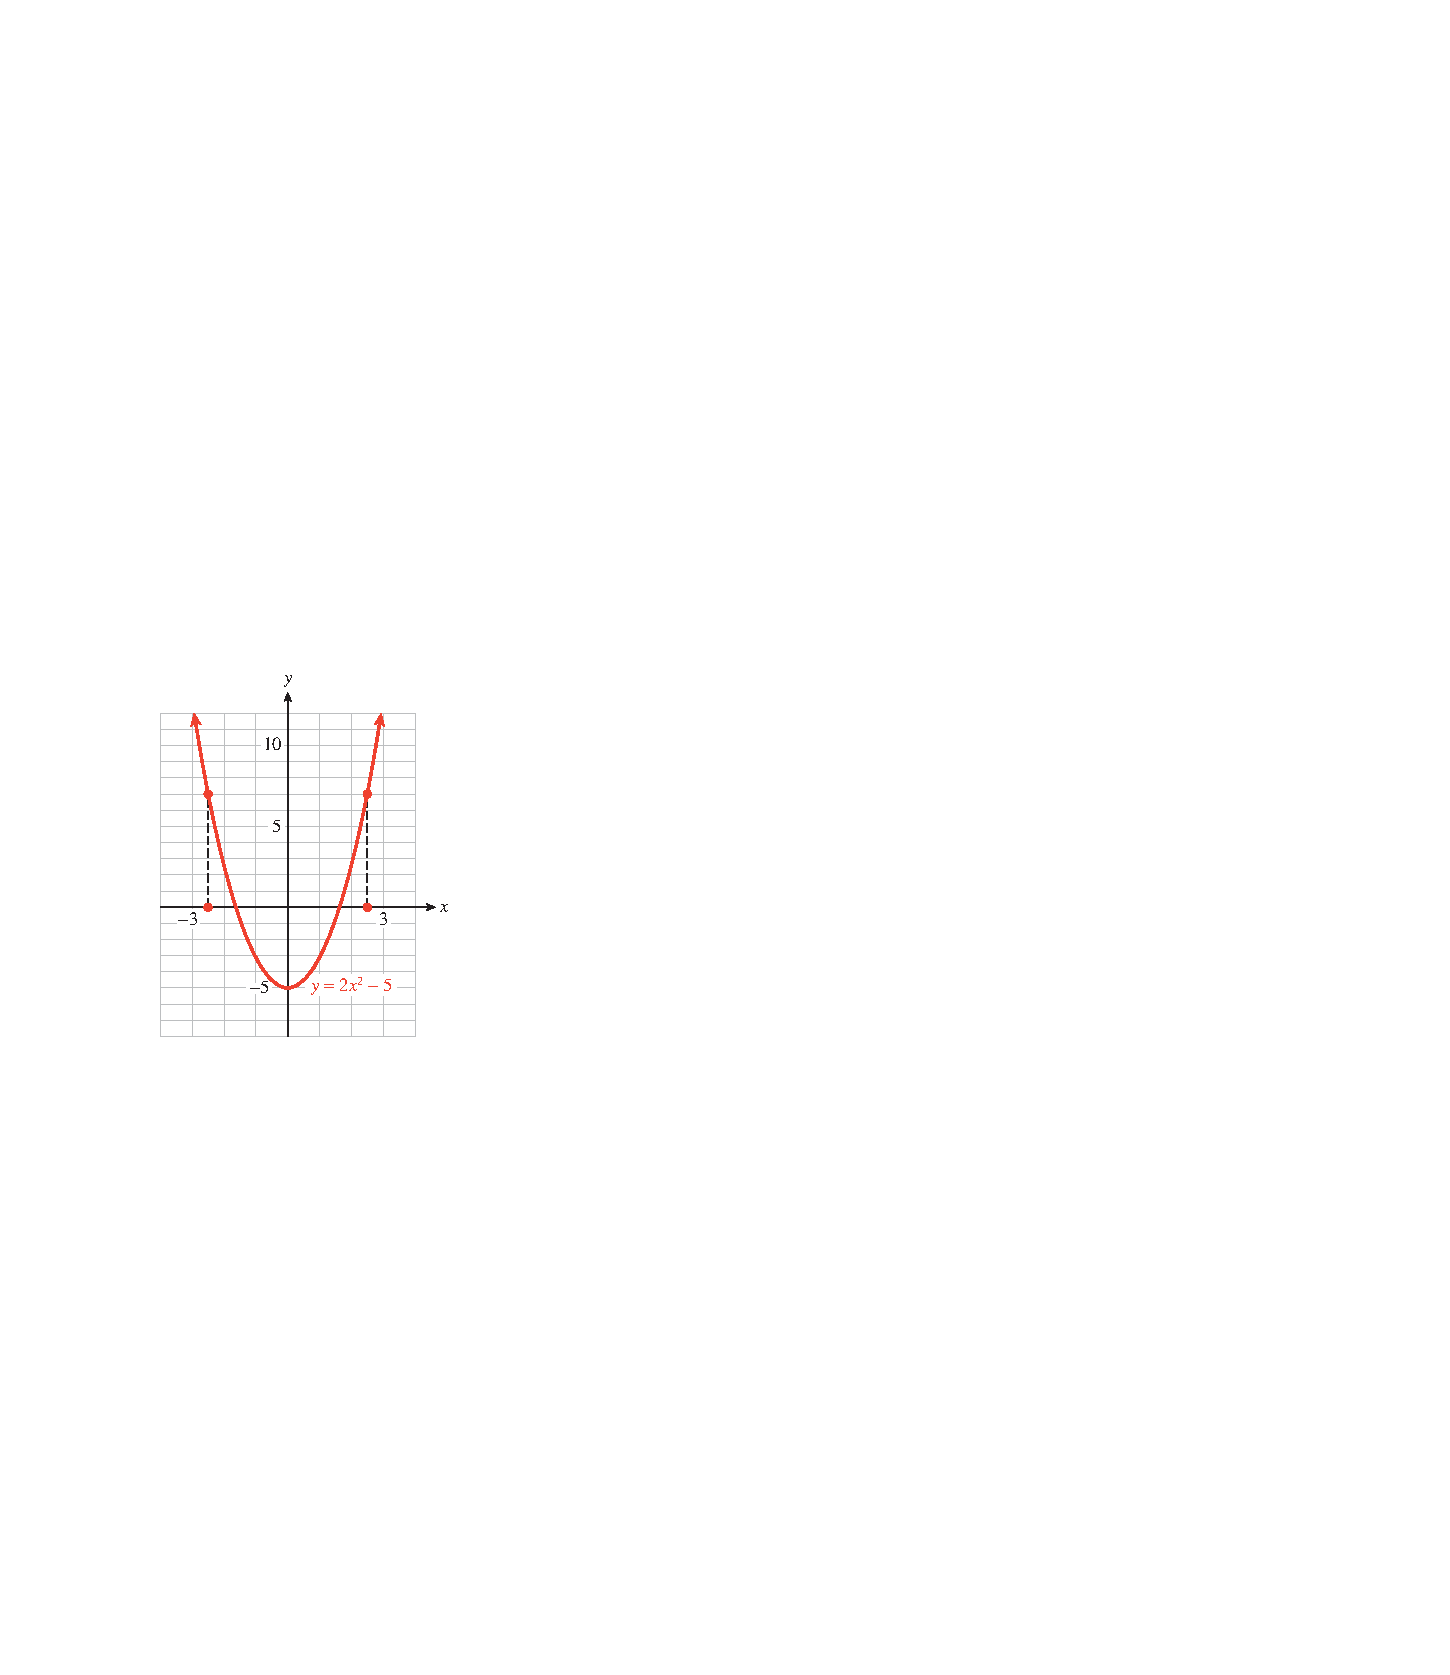
\includegraphics[width=\textwidth,]{images/fig-parabola.pdf}}% end body 
{\captionof{figure}{\label{fig-parabola}}
}% caption 
\pushValignCaptionBottom[b]{minipage}{.50\textwidth}{%
\parbox{\textwidth}{%
% horizontal alignment 

    When studying nonlinear models, we will need to solve nonlinear equations. For example, in Investigation 3 we used a graph to solve the quadratic equation 
    \begin{equation*}18x − x^2 = 80\end{equation*} 
    Here is another example. \hyperref[fig-parabola]{Figure~\ref{fig-parabola}} shows a table and graph for the function \(y = 2x^2 − 5\).
}%
}% end body 
{}% caption 
\popValignCaptionBottom
\end{figure}
\leavevmode%
\begin{table}
\centering
\begin{tabular}{AcAcAcAcAcAcAcAcA}\hrulethick
\(x\)&\(-3\)&\(-2\)&\(-1\)&\(0\)&\(1\)&\(2\)&\(3\)\tabularnewline\hrulethin
\(y\)&\(13\)&\(3\)&\(-3\)&\(-5\)&\(-3\)&\(3\)&\(13\)\tabularnewline\hrulethin
\end{tabular}
\end{table}

    You can see that there are two points on the graph for each \(y\)-value greater than \(−5\). For example, the two points with \(y\)-coordinate \(7\) are shown. To solve the equation 
    \begin{equation*}2x^2 − 5 = 7\end{equation*} 
    we need only find the x-coordinates of these points. From the graph, the solutions appear to be about 2.5 and −2.5.
%
\par

    How can we solve this equation algebraically? The opposite operation for squaring a number is taking a square root. So we can undo the operation of squaring by extracting square roots. We first solve for \(x^2\) to get
    \begin{align}
    2x^2 \amp= 12 \\
    x^2 \amp= 6\\
    \end{align}
    and then take square roots to find
    \begin{equation*}x = \pm\sqrt{6}\end{equation*}
%
\par

    Don't forget that every positive number has two square roots. The symbol \(\pm\) (read “plus or minus”) is a shorthand notation used to indicate both square roots of \(6\). The exact solutions are thus \(\sqrt{6}\) and \(-\sqrt{6}\). We can also find decimal approximations for the solutions using a calculator. Rounded to two decimal places, the approximate solutions are \(2.45\) and \(−2.45\).
%
\par

    In general, wecan solve equations of the form 
    \(ax^2 + c = 0\)
    by isolating \(x^2\) on one side of the equation and then taking the square root of each side. This method for solving equations is called \terminology{extraction of roots}.
%
\typeout{************************************************}
\typeout{Paragraphs  Extraction of Roots}
\typeout{************************************************}
\paragraph[Extraction of Roots]{Extraction of Roots}\label{paragraphs-1}

    To solve the equation
    \begin{equation*}ax^2 + c = 0\end{equation*}
    \leavevmode%
\begin{enumerate}
\item\hypertarget{li-1}{}Isolate \(x^2\).\item\hypertarget{li-2}{}Take square roots of both sides. There are two solutions.\end{enumerate}

%
\begin{example}[]\label{example-cat-falling}

        If a cat falls off a tree branch 20 feet above the ground, its height t seconds later is given by \(h = 20 − 16t^2\).
    %
\leavevmode%
\begin{enumerate}[label=*\alph**]
\item\hypertarget{li-3}{}What is the height of the cat \(0.5\) second later?\item\hypertarget{li-4}{}How long does the cat have to get in position to land on its feet before it reaches the ground?\end{enumerate}
\par\medskip\noindent%
\textbf{Solution.}\quad \leavevmode%
\begin{enumerate}[label=*\alph**]
\item\hypertarget{li-5}{}In this question, we are given the value of \(t\) and asked to find the corresponding value of \(h\). To do this, we evaluate the formula for \(t = 0.5\). We substitute \(\alert{0.5}\) for \(t\) into the formula and simplify.
    \begin{align*}
    h \amp= 20 − 16(\alert{0.5})^2 \amp\amp \text{Compute the power.}\\
    \amp = 20 − 16 (0.25) \amp\amp \text{Multiply; then subtract.}\\
    \amp = 20 − 4 = 16
    \end{align*}
    The cat is \(16\) feet above the ground after \(0.5\) second.\item\hypertarget{li-6}{}We would like to find the value of \(t\) when the height, \(h\), is known. We substitute \(h = \alert{0}\) into the equation to obtain
    \begin{equation*}\alert{0} = 20 − 16t^2\end{equation*}
    To solve this equation, we use extraction of roots. First isolate \(t^2\) on one side of the equation.
    \begin{align*}
    16t^2 \amp= 20 \amp\amp \text{Divide by 16.}\\
    t^2 \amp= \frac{20}{16}=1.25
    \end{align*}
    Now take the square root of both sides of the equation to find
    \begin{equation*}t = \pm \sqrt{1.25} \approx \pm1.118\end{equation*}\end{enumerate}
\end{example}
\leavevmode%
\begin{figure}
\centering
\pushValignCaptionBottom[b]{minipage}{.50\textwidth}{%
\centering% horizontal alignment 
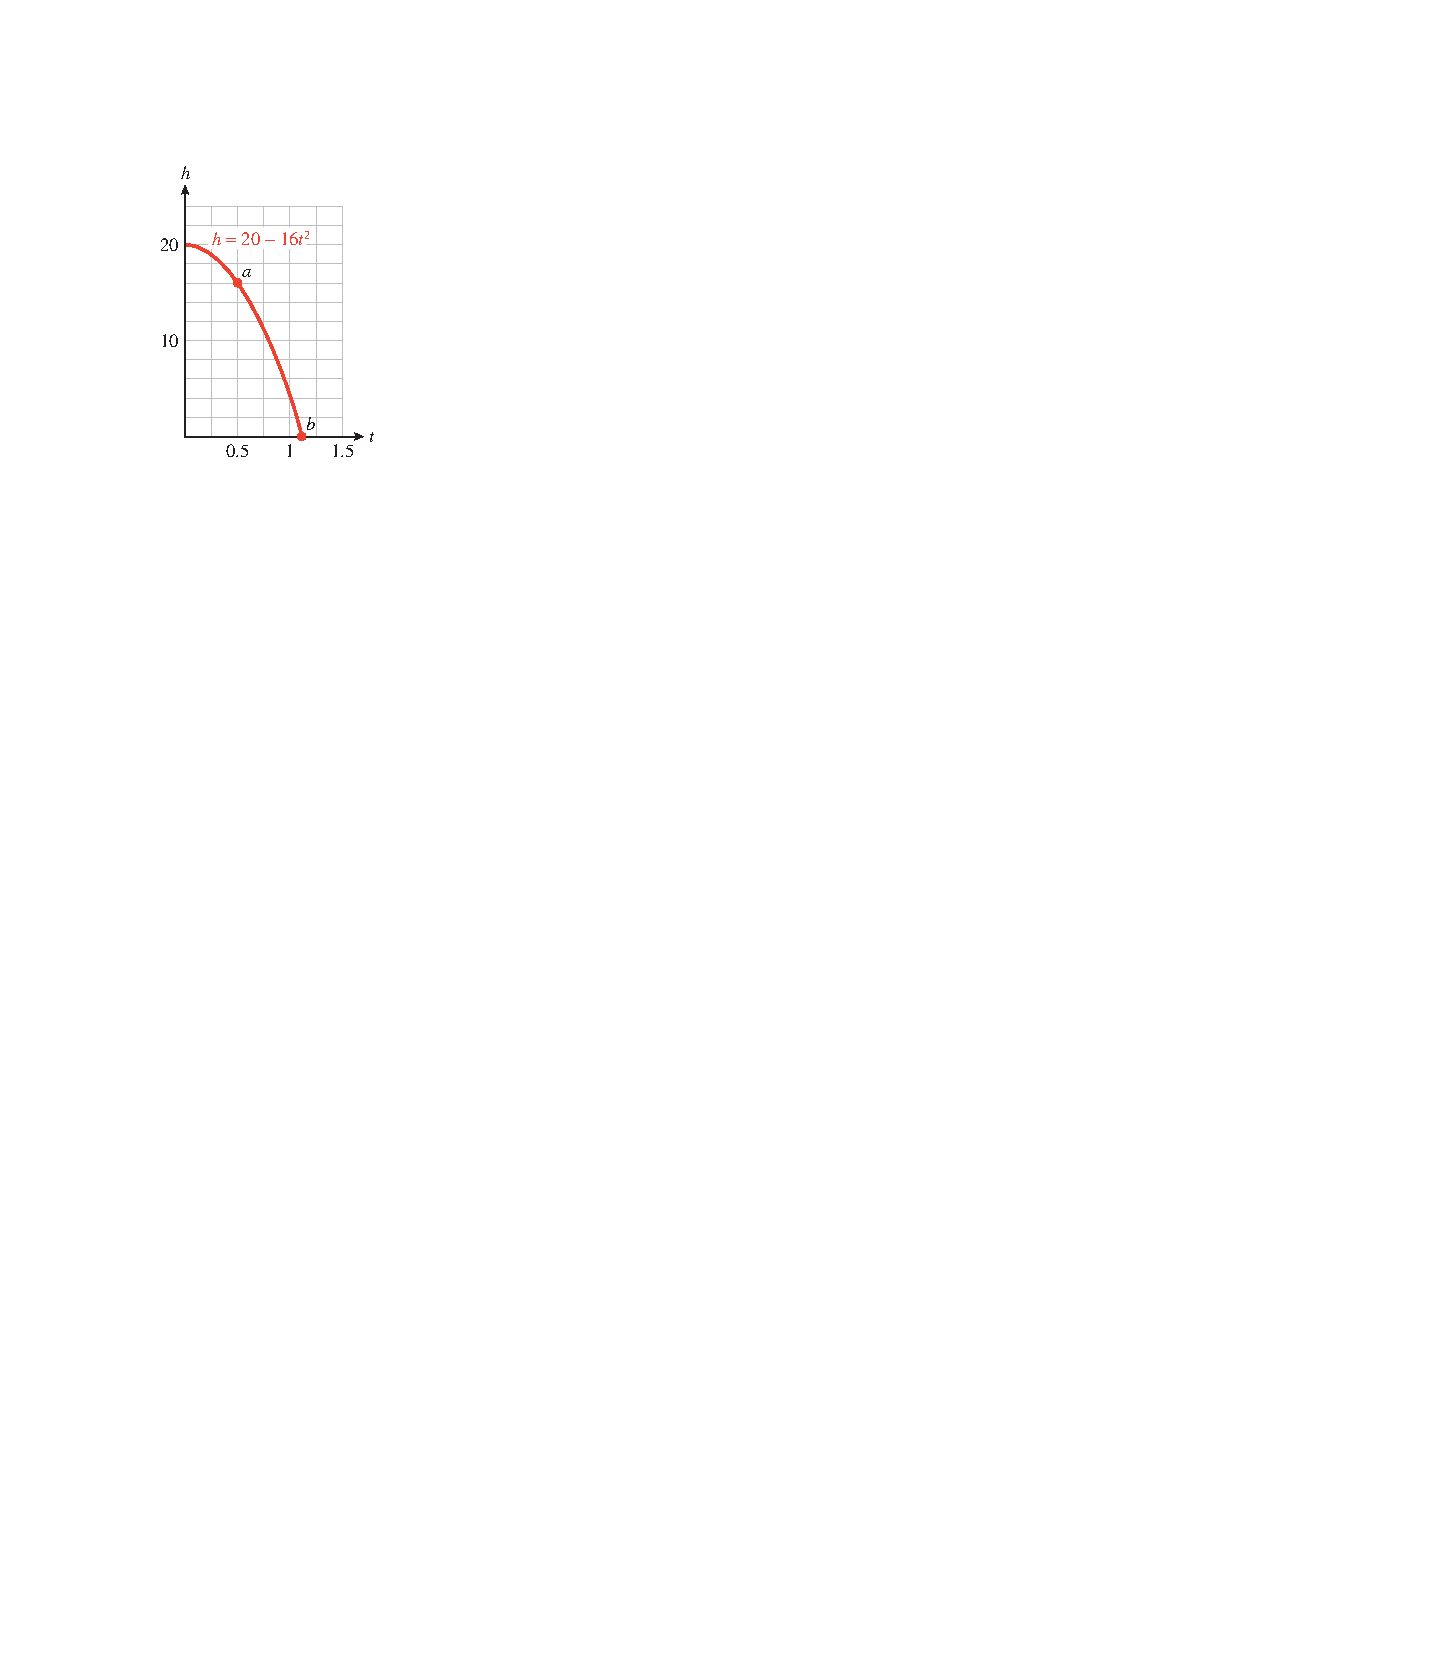
\includegraphics[width=\textwidth,]{images/fig-cat-falling.pdf}}% end body 
{\captionof{figure}{\label{fig-cat-falling}}
}% caption 
\pushValignCaptionBottom[b]{minipage}{.50\textwidth}{%
\parbox{\textwidth}{%
% horizontal alignment 

    Only the positive solution makes sense here, so the cat has approximately 1.12 seconds to get into position for landing. A graph of the cat’s height after t seconds is shown in Figure 2.3. The points corresponding to parts (a) and (b) are labeled.
}%
}% end body 
{}% caption 
\popValignCaptionBottom
\end{figure}
\par

    Note that in \hyperref[example-cat-falling]{Example~\ref{example-cat-falling}} we evaluated the expression \(20 − 16t^2\) to find a value for \(h\), and in part (b) we solved the equation \(0 = 20 − 16t^2\) to find a value for \(t\).
%
\begin{exercise}\label{exercise-extract-roots}
\leavevmode%
\begin{enumerate}[label=*\alph**]
\item\hypertarget{li-7}{}\leavevmode%
\begin{figure}
\centering
\pushValignCaptionBottom[b]{minipage}{.50\textwidth}{%
\parbox{\textwidth}{%
% horizontal alignment 
Solve by extracting roots
            \(\frac{3x^2 − 8}{5}= 10\).}%
}% end body 
{}% caption 
\pushValignCaptionBottom[b]{minipage}{.50\textwidth}{%
\parbox{\textwidth}{%
% horizontal alignment 
First, isolate \(x^2\).Take the square root of both sides.}%
}% end body 
{}% caption 
\popValignCaptionBottom
\end{figure}
\item\hypertarget{li-8}{}Give exact answers; then give approximations rounded to two decimal places.\end{enumerate}
\end{exercise}
\typeout{************************************************}
\typeout{Subsection  Solving Formulas}
\typeout{************************************************}
\subsection[Solving Formulas]{Solving Formulas}\label{subsection-2}

    We can use extraction of roots to solve many formulas involving the square of the variable.
%
\begin{example}[]\label{example-volume-cone}
The formula \(V = \frac{1}{3} πr^2h\) gives the volume of a cone in terms of its height and radius. Solve the formula for \(r\) in terms of \(V\) and \(h\).
    %
\par\medskip\noindent%
\textbf{Solution.}\quad 
    Because the variable we want is squared, we use extraction of roots. First, multiply both sides by \(3\) to clear the fraction.
    \begin{equation*}
        \begin{aligned}
        3V \amp = 3(\frac{1}{3} πr^2h)\\
        3V \amp = πr^2h \amp\amp \text{Divide both sides by } πh.\\
        \frac{3V}{πh}\amp= r^2 \amp\amp \text{Take square roots.}\\
        \pm\sqrt{\frac{3V}{πh}}\amp= r
        \end{aligned}
    \end{equation*}
    Because the radius of a cone must be a positive number, we use only the positive square root: 
    \(r = \sqrt{\frac{3V}{πh}}\).
\end{example}
\begin{exercise}\label{exercise-area-circle}
Find a formula for the radius of a circle in terms of its area.%
Start with the formula for the area of a circle: \(A =\) \fillin{3.636363636363636}%
\par
Solve for \(r\) in terms of \(A\).%
\end{exercise}
\typeout{************************************************}
\typeout{Subsection  More Extraction of Roots}
\typeout{************************************************}
\subsection[More Extraction of Roots]{More Extraction of Roots}\label{subsection-3}

    Equations of the form
    \begin{equation*}a( px + q)^2 + r = 0\end{equation*}
    can also be solved by extraction of roots after isolating the squared expression, \((px + q)^2\).
%
\begin{example}[]\label{example-extracting-roots}

    Solve the equation \(3(x − 2)^2 = 48\).
%
\par\medskip\noindent%
\textbf{Solution.}\quad 
    First, isolate the perfect square, \((x − 2)^2\).
    \begin{equation*}
        \begin{aligned}
        3(x − 2)^2 \amp = 48 \amp\amp\text{Divide both sides by }3.\\
        (x − 2)^2 \amp = 16 \amp\amp\text{Take the square root of each side.}\\
        x − 2 \amp = \pm\sqrt{16} = \pm 4
        \end{aligned}
    \end{equation*}
    
    This gives us two equations for \(x\), 
    \begin{equation*}
        \begin{aligned}
        x − 2 \amp =4 \amp\amp \text{or }\amp x − 2 \amp =−4\amp\amp\text {Solve each equation.}\\
        x \amp=6 \amp\amp \text{or }\amp x \amp =−2
        \end{aligned}
    \end{equation*}
        The solutions are \(6\) and \(−2\).
\end{example}
\typeout{************************************************}
\typeout{Paragraphs  Extraction of Roots}
\typeout{************************************************}
\paragraph[Extraction of Roots]{Extraction of Roots}\label{paragraphs-2}

    To solve the equation
    \begin{equation*}a(px+q)^2 +r=0\end{equation*}
%
\leavevmode%
\begin{enumerate}
\item\hypertarget{li-9}{}Isolate the squared expression, \((px + q)^2\).\item\hypertarget{li-10}{}Take the square root of each side of the equation. Remember that a positive number has two square roots.\item\hypertarget{li-11}{}Solve each equation. There are two solutions.\end{enumerate}
\begin{exercise}\label{exercise-extract-roots2}

    Solve \(2(5x + 3)^2 = 38\) by extracting roots.
    \leavevmode%
\begin{enumerate}[label=*\alph**]
\item\hypertarget{li-12}{}Give your answers as exact values.\item\hypertarget{li-13}{}Find approximations for the solutions to two decimal places.\end{enumerate}
\end{exercise}
\typeout{************************************************}
\typeout{Subsection  Compound Interest and Inflation}
\typeout{************************************************}
\subsection[Compound Interest and Inflation]{Compound Interest and Inflation}\label{subsection-4}

    Many savings institutions offer accounts on which the interest is \emph{compounded annually}. At the end of each year, the interest earned is added to the principal, and the interest for the next year is computed on this larger sum of money.
%
\typeout{************************************************}
\typeout{Paragraphs  Compound Interest}
\typeout{************************************************}
\paragraph[Compound Interest]{Compound Interest}\label{paragraphs-3}

    If interest is compounded annually for \(n\) years, the amount, \(A\), of money in an account is given by
    \begin{equation*}A = P(1 + r)^n\end{equation*}
    where \(P\) is the principal and \(r\) is the interest rate, expressed as a decimal fraction.
%
\begin{example}[]\label{example-compound-interest}

    Carmella invests \textdollar{}3000 in an account that pays an interest rate, \(r\), compounded annually.
    \leavevmode%
\begin{enumerate}[label=*\alph**]
\item\hypertarget{li-14}{}Write an expression for the amount of money in Carmella’s account after two years.\item\hypertarget{li-15}{}What interest rate would be necessary for Carmella's account to grow to \textdollar{}3500 in two years?\end{enumerate}

%
\par\medskip\noindent%
\textbf{Solution.}\quad \leavevmode%
\begin{enumerate}[label=*\alph**]
\item\hypertarget{li-16}{}Use the formula above with \(P = 3000\) and \(n = 2\). Carmella’s account balance will be
            \begin{equation*}A = 3000(1 + r)^2\end{equation*}\item\hypertarget{li-17}{}Substitute \(3500\) for \(A\) in the equation.
        \begin{equation*}\alert{3500} = 3000(1 + r)^2\end{equation*}
        We can solve this equation in \(r\) by extraction of roots. First, isolate the perfect square.
        \begin{align}
        3500 \amp = 3000(1 + r )^2 \amp\amp \text{Divide both sides by 3000.} \\
        1.1\overline{6} \amp = (1 + r )^2 \amp\amp \text{Take the square root of both sides.} \\
        \pm 1.0801 \amp\approx 1 + r \amp\amp \text{Subtract 1 from both sides.}
        r \amp\approx 0.0801 \amp\amp \text{or }\amp r \approx −2.0801
        \end{align}
        Because the interest rate must be a positive number, we discard the negative solution. Carmella needs an account with interest rate \(r \approx 0.0801\), or just over 8\%, to achieve an account balance of \textdollar{}3500 in two years.\end{enumerate}
\end{example}
\par

    The formula for compound interest also applies to the effects of inflation. For instance, if there is a steady inflation rate of 4\% per year, in two years an item that now costs \textdollar{}100 will cost
    \begin{align}
    A \amp= P(1 + r)^2\\
    \amp = 100(1 + 0.04)2 = \$108.16
    \end{align}
%
\begin{exercise}\label{exercixe-inflation}

    Two years ago, the average cost of dinner and a movie was \textdollar{}24. This year the average cost is \textdollar{}25.44. What was the rate of inflation over the past two years?
\end{exercise}
\typeout{************************************************}
\typeout{Subsection  Other Nonlinear Equations}
\typeout{************************************************}
\subsection[Other Nonlinear Equations]{Other Nonlinear Equations}\label{subsection-5}

    Because squaring and taking square roots are opposite operations, we can solve the equation
    \begin{equation*}\sqrt{x} = 8.2\end{equation*}
    by squaring both sides to get
    \begin{align}
    (\sqrt{x})^2 \amp= 8.2^2 \\
    x \amp = 67.24
    \end{align}
    Similarly, we can solve
    \begin{equation*}x^3 = 258\end{equation*}
    by taking the cube root of both sides, because cubing and taking cube roots are opposite operations. Rounding to three places, we find 
    \begin{align}
    \sqrt[3]{x^3}\amp=258\\
    x \amp \approx 6.366
    \end{align}
    The notion of undoing operations can help us solve a variety of simple nonlinear equations. The operation of taking a reciprocal is its own opposite, so we solve the equation
    \begin{equation*}\frac{1}{x} = 50\end{equation*}
    by taking the reciprocal of both sides to get
    \begin{equation*}x = \frac{1}{50}= 0.02\end{equation*}
%
\begin{example}[]\label{example-nonlinear-equation}

        Solve \(\frac{3}{x − 2}= 4\).
    %
\par\medskip\noindent%
\textbf{Solution.}\quad 
    We begin by taking the reciprocal of both sides of the equation to get
    \begin{equation*}\frac{x − 2}{3}= \frac{1}{4}\end{equation*}
    We continue to undo the operations in reverse order. Multiply both sides by \(3\).
    \begin{align}
    x − 2 \amp = \frac{3}{4} \amp\amp \text{Add 2 to both sides.}\\
    x \amp = 2 + \frac{3}{4}= \frac{11}{4} \amp\amp \frac{2}{1}=\frac{8}{4}
    \text{, so } \frac{2}{1}+ \frac{3}{4}=\frac{8}{4}+\frac{3}{4}=\frac{11}{4}
    \end{align}
    The solution is \(\frac{11}{4}\), or \(2.75\).
\end{example}
\begin{exercise}\label{exercise-nonlinear-equation}

    Solve \(2\sqrt{x + 4} = 6\).
\end{exercise}
\begin{remark}[
\includegraphics[width=0.8\textwidth,]{images/icon-GC.pdf}Using the Intersect Feature]\label{remark-1}
We can use the \emph{intersect} feature on a graphing calculator to solve equations.%
\end{remark}
\begin{example}[]\label{example-GC-nonlinear-equation}

        Use a graphing calculator to solve \(\frac{3}{x −2}= 4.\)
    %
\par\medskip\noindent%
\textbf{Solution.}\quad 
    We would like to find the points on the graph of \(y = \frac{3}{x −2}\) that have \(y\)-coordinate equal to \(4\). Graph the two functions
    \begin{align}
    Y_1 \amp = 3/(X − 2)  \\
    Y_2 \amp = 4
    \end{align}

    in the window
    \begin{align}
    \text{Xmin} \amp = −9.4 \amp\amp \text{Xmax} = 9.4\\
    \text{Ymin} \amp = −10 \amp\amp \text{Ymax} = 10
    \end{align}
    The point where the two graphs intersect locates the solution of the equation. If we trace along the graph of \(Y_1\), the closest we can get to the intersection point is \((2.8, 3.75)\), as shown in \hyperref[fig-GC-nonlinear]{Figure~\ref{fig-GC-nonlinear}}a. We get a better approximation using the \emph{intersect} feature.
    \leavevmode%
\begin{figure}
\centering
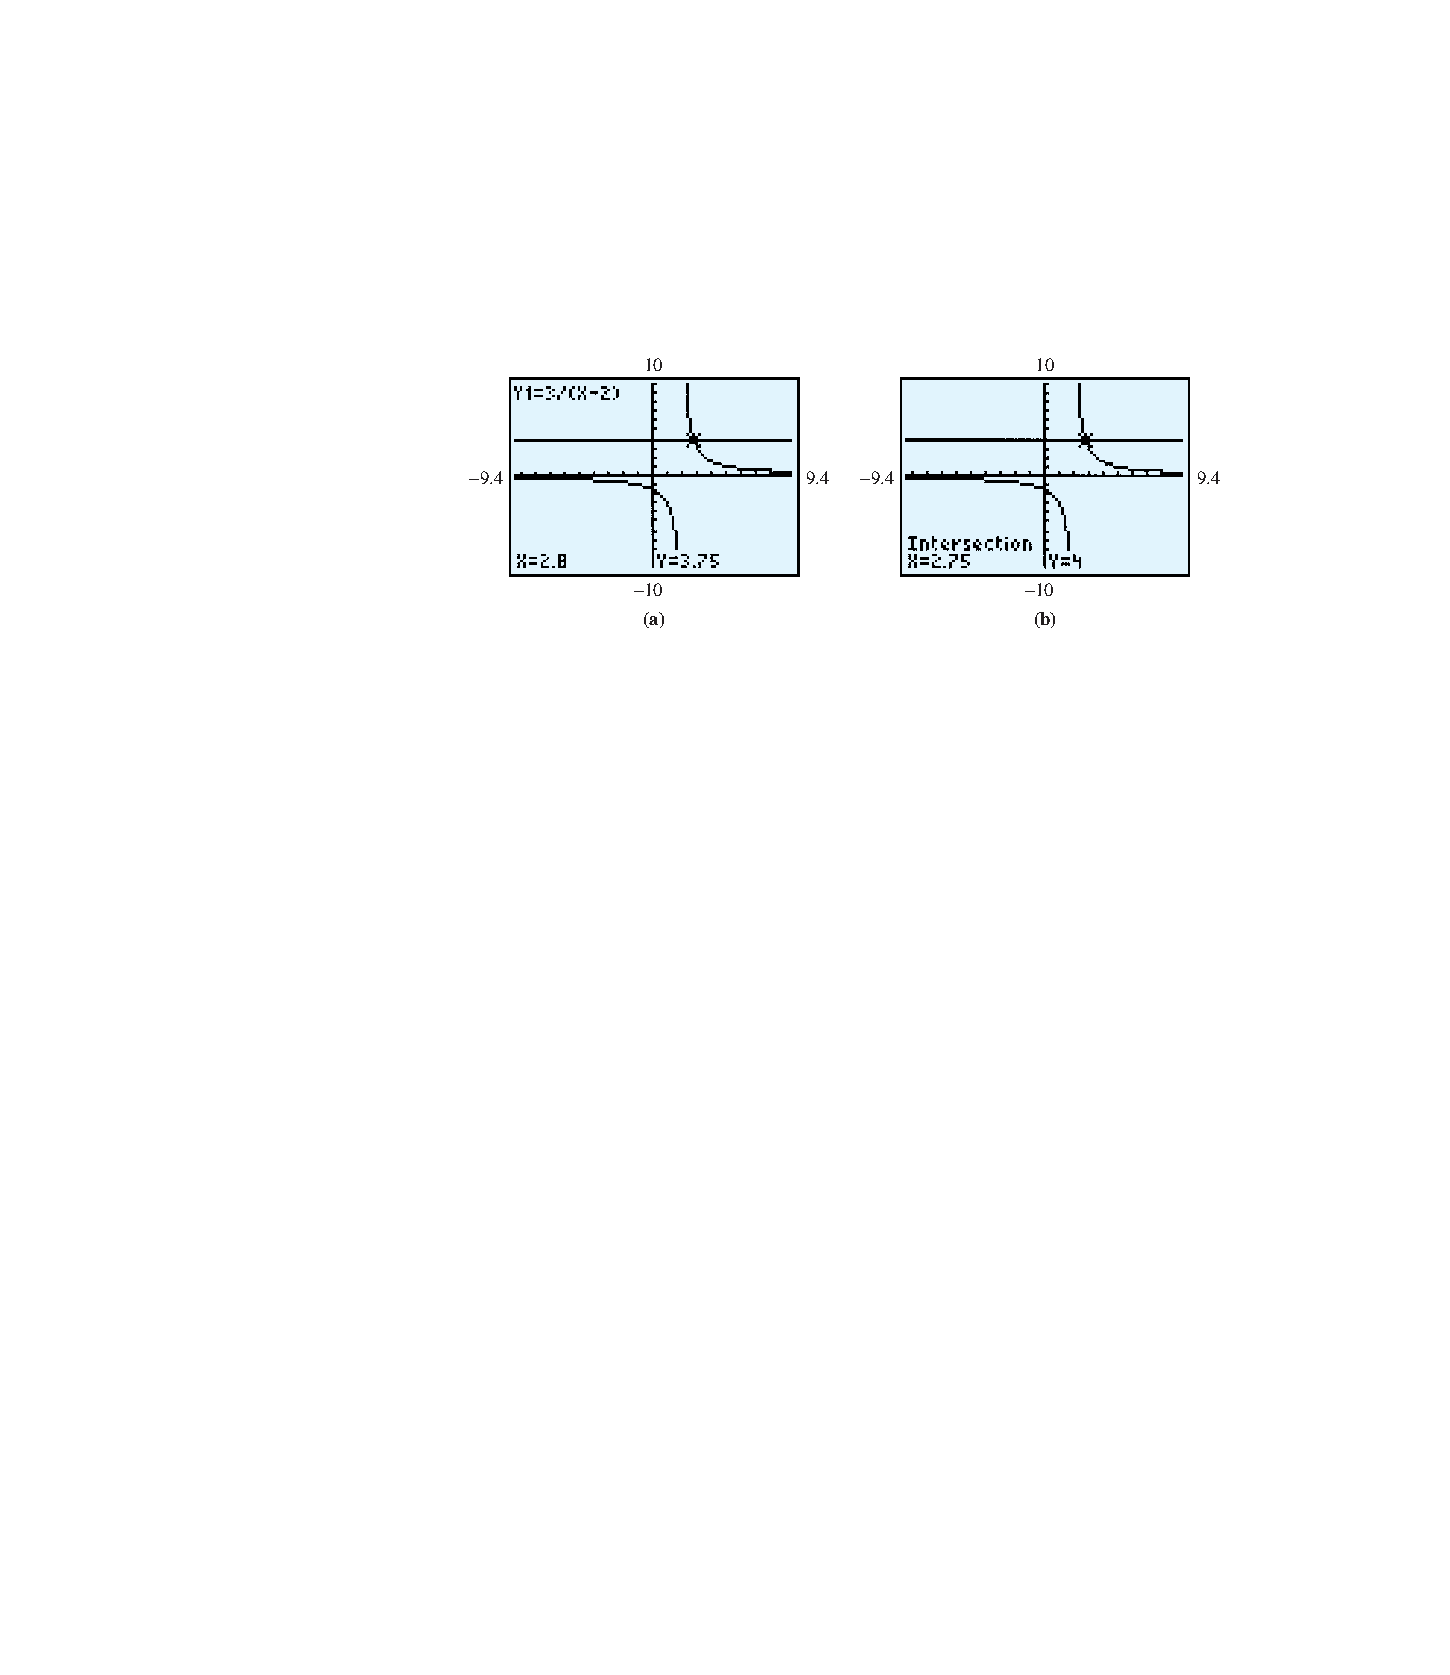
\includegraphics[width=0.100\textwidth,]{images/fig-GC-nonlinear.pdf}\caption{\label{fig-GC-nonlinear}}
\end{figure}


    Use the arrow keys to position the Trace bug as close to the intersection point as you can. Then press 
\includegraphics[width=0.6\textwidth,]{images/icon-2nd.pdf}
\includegraphics[width=0.12\textwidth,]{images/icon-trace.pdf} to see the Calculate menu. Press \(5\) for intersect; then respond to each of the calculator's questions, \emph{First curve?}, \emph{Second curve?}, and \emph{Guess?} by pressing 
\includegraphics[width=0.11\textwidth,]{images/icon-enter.pdf}. The calculator will then display the intersection point, \(x = 2.75\), \(y = 4\), as shown in \hyperref[fig-GC-nonlinear]{Figure~\ref{fig-GC-nonlinear}}b. The solution of the original equation is \(x = 2.75\).
\end{example}
\begin{exercise}\label{exercise-GC-nonlinear}

    Use the intersect feature to solve the equation \(2x^2 − 5 = 7\). Round your answers to three decimal places.
\end{exercise}
\typeout{************************************************}
\typeout{Section 1.2 Solving Quadratic Equations}
\typeout{************************************************}
\section[Solving Quadratic Equations]{Solving Quadratic Equations}\label{Solving-Quadratic-Equations}

	Not every quadratic equation can be solved by factoring or by extraction of roots. For example, the expression \(x^2 + x − 1\) cannot be factored, so the equation \(x^2 + x − 1 = 0\) cannot be solved by factoring. For other equations, factoring may be difficult. In this section we learn two methods that can be used to solve any quadratic equation.
%
\typeout{************************************************}
\typeout{Subsection  Squares of Binomials}
\typeout{************************************************}
\subsection[Squares of Binomials]{Squares of Binomials}\label{subsection-6}

	In \hyperref[nonlinear-models]{Section~\ref{nonlinear-models}} we used extraction of roots to solve equations of the form 
	\begin{equation*}a( px + q)^2 + r = 0\end{equation*}
	where the left side of the equation includes the square of a binomial, or a \terminology{perfect square}. We can write any quadratic equation in this form by completing the square.
%
\par

	Consider the following squares of binomials.
%
\leavevmode%
\begin{table}
\centering
\begin{tabular}{AcAcAcAcA}\hrulethick
Square of binomial \((x+p)^2\)&\(p\)&\(2p\)&\(p^2\)\tabularnewline\hrulethick
1.  \((x+\alert{5})^2=x^2+10x+25\)&\(\alert{5}\)&\(2(\alert{5})=10\)&\(\alert{5}^2=25\)\tabularnewline\hrulethin
2.  \((x\alert{{}-{}3})^2=x^2-6x+9\)&\(\alert{-3}\)&\(2(\alert{-3})=-6\)&\(\alert{-3}^2=9\)\tabularnewline\hrulethin
3.  \((x\alert{{}-{}12})^2=x^2-24x+144\)&\(\alert{-12}\)&\(2(\alert{-12})=-24\)&\(\alert{-12}^2=144\)\tabularnewline\hrulethin
\end{tabular}
\end{table}
\par

	In each case, the square of the binomial is a quadratic trinomial,
	\begin{equation*}(x + p)^2= x^2 + 2px + p^2\end{equation*}
	The coefficient of the linear term, \(2p\), is twice the constant in the binomial, and the constant term of the trinomial, \(p^2\), is its square.
%
\par

	We would like to reverse the process and write a quadratic expression as the square of a binomial. For example, what constant term can we add to
	\begin{equation*}x^2 − 16x\end{equation*}
	to produce a perfect square trinomial? Compare the expression to the formula above:
	\begin{equation*}
		\begin{alignedat}{4}
		x^2 \amp {}+{} \amp 2px \amp {}+{} \amp p^2 \amp {}={} \amp (x + p)^2 \\
		x^2 \amp {}-{} \amp 16x \amp {}+{} \amp \text{?} \amp {}={} \amp (x + \text{?})^2 \\
		\end{alignedat}
	\end{equation*}
	We see that \(2p = −16\), so \(p = \frac{1}{2}(−16) = −8\), and \(p^2 = (−8)^2 = 64\). Substitute these values for \(p^2\) and \(p\) into the equation to find
	\begin{equation*}x^2 − 16x + 64 = (x − 8)^2\end{equation*}
	Notice that in the resulting trinomial, the constant term is equal to \emph{the square of one-half the coefficient of} \(x\). In other words, we can find the constant term by taking one-half the coefficient of \(x\) and then squaring the result. Adding a constant term obtained in this way is called \terminology{completing the square}.
%
\begin{example}[]\label{example-completing-the-square}

		Complete the square by adding an appropriate constant; write the result as the square of a binomial.
		\leavevmode%
\begin{enumerate}[label=*\alph**]
\item\hypertarget{li-18}{}\(x^2 − 12x + {}\)\fillin{2.727272727272727}\item\hypertarget{li-19}{}\(x^2 + 5x + {}\)\fillin{2.727272727272727}\end{enumerate}

	%
\par\medskip\noindent%
\textbf{Solution.}\quad \leavevmode%
\begin{enumerate}[label=*\alph**]
\item\hypertarget{li-20}{}
			One-half of \(−12\) is \(−6\), so the constant term is \((−6)^2\), or \(36\). Add \(36\) to obtain
			\begin{equation*}x^2 − 12x \alert{{}+{}36}=(x − 6)^2~~~~~~~  \underset{p^2 = (−6)^2 = 36}{\stackrel {p = \frac{1}{2}(−12) = −6}{}}\end{equation*}\item\hypertarget{li-21}{}
			One-half of \(5\) is \(\frac{5}{2}\), so the constant term is \(\left(\frac{5}{2}\right)^2\), or \(\frac{25}{4}\). Add \(\frac{25}{4}\) to obtain
			\begin{equation*}x^2 +5x \alert{{}+{}\frac{25}{4}}=\left(x +\frac{5}{2}\right)^2~~~~~~~  \underset{p^2 = (\frac{5}{2})^2 = \frac{25}{4}}{\stackrel {p = \frac{1}{2}(5) = \frac{5}{2}}{}}\end{equation*}\end{enumerate}

	%
\end{example}
\par

	You may find it helpful to visualize completing the square geometrically. We can think of the expression \(x^2 + 2px\) as the area of a rectangle with dimensions \(x\) and \(x + 2p\). For example, the rectangle with length \(x + 10\) and width \(x\) has area \(x(x + 10) = x^2 + 10x\), as shown in \hyperref[fig-completing-the-square]{Figure~\ref{fig-completing-the-square}}a. We would like to cut the rectangle into pieces and rearrange them so that we can make a square. In \hyperref[fig-completing-the-square]{Figure~\ref{fig-completing-the-square}}b, we move half of the \(x\)-term so that each side of the square has length \(x + 5\) (note that \(p = \frac{1}{2} (10) = 5\)), and in \hyperref[fig-completing-the-square]{Figure~\ref{fig-completing-the-square}}c we see that the missing corner piece has area \(p^2 = 5^2 = 25\).
%
\leavevmode%
\begin{figure}
\centering
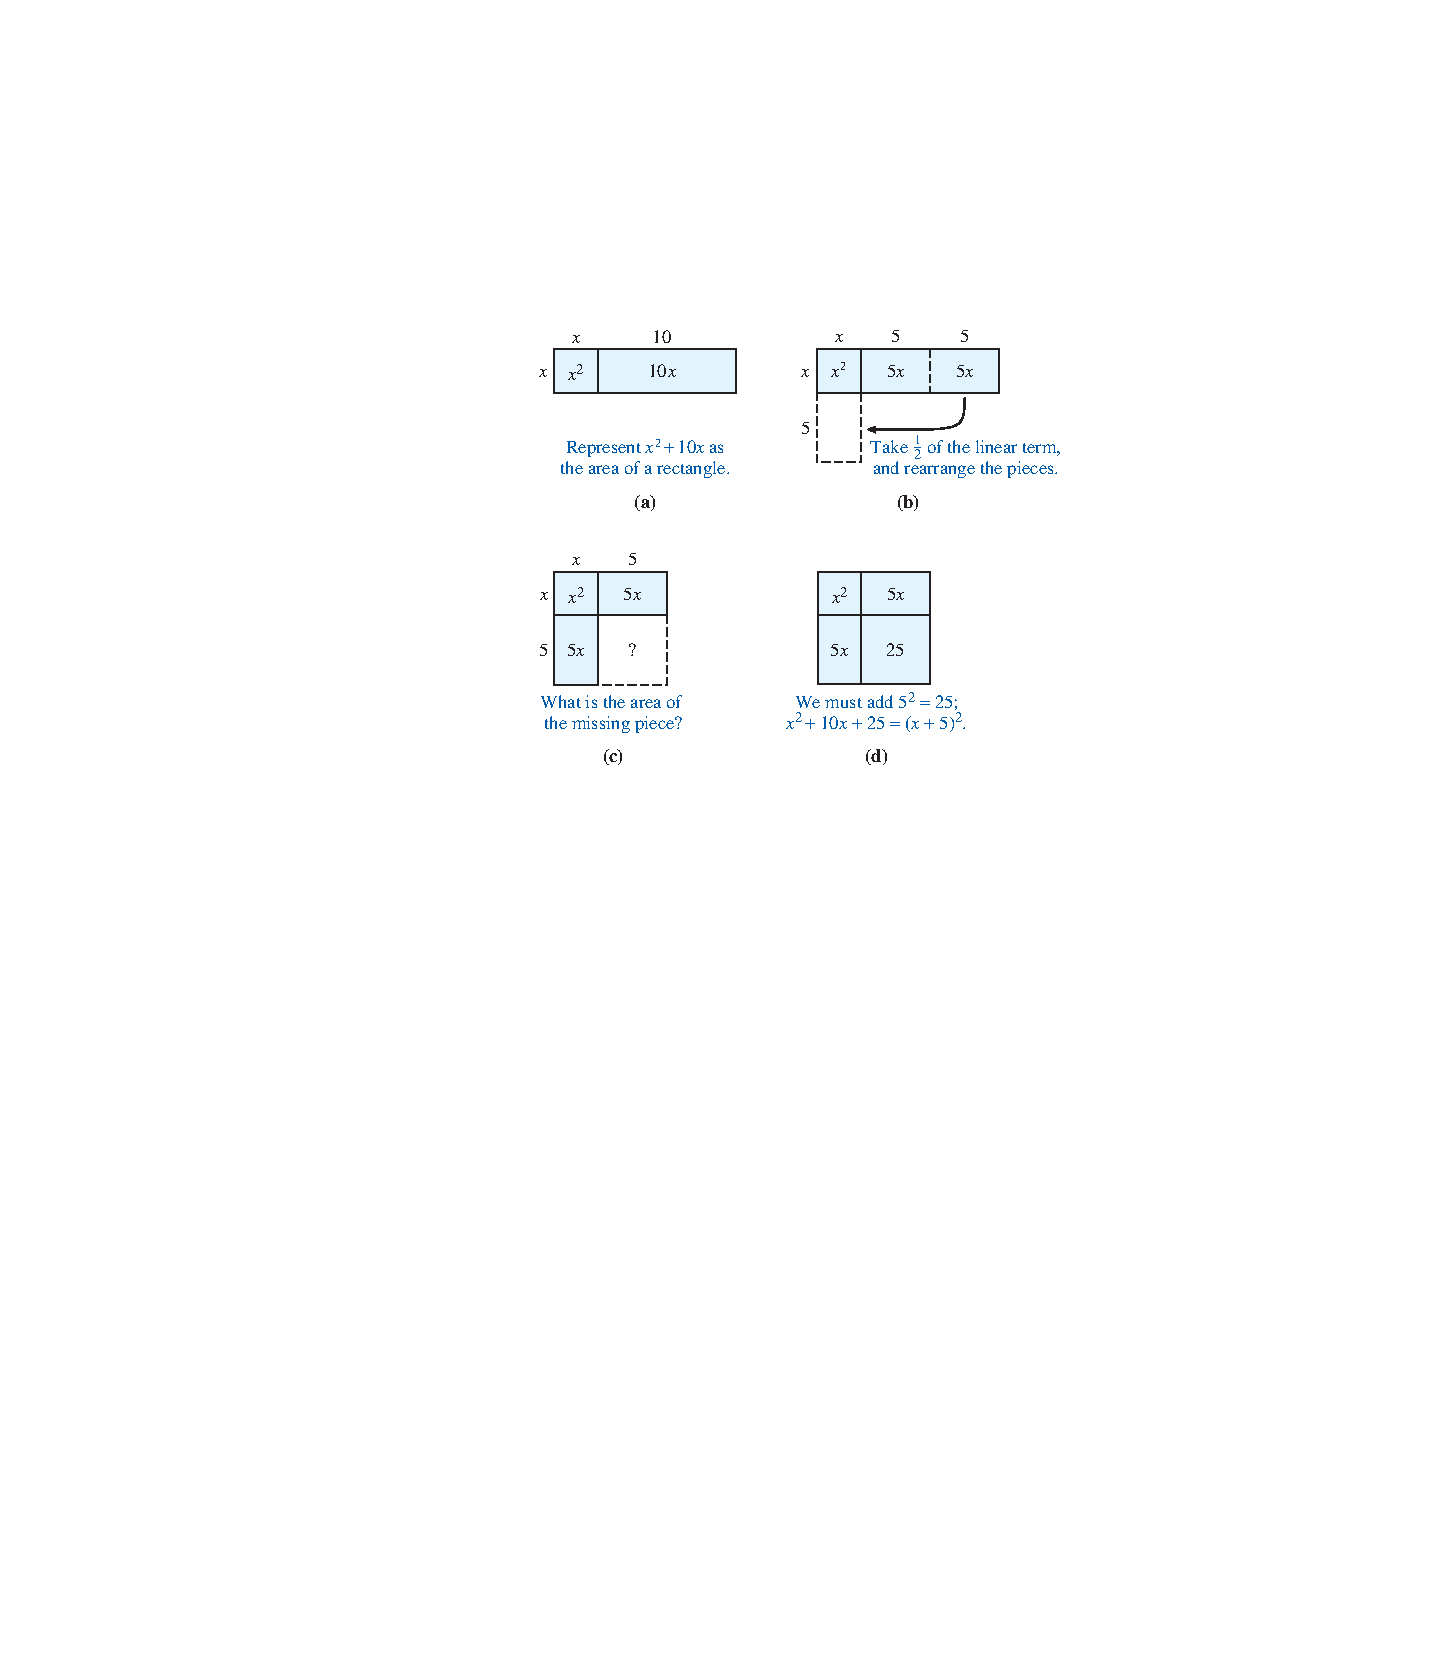
\includegraphics[,]{images/fig-completing-the-square.pdf}\caption{\label{fig-completing-the-square}}
\end{figure}
\begin{exercise}\label{exercise-completing-the-square}

		Complete the square by adding an appropriate constant; write the result as the square of a binomial.
		\leavevmode%
\begin{enumerate}[label=*\alph**]
\item\hypertarget{li-22}{}\(x^2 − 18x{} + {}\)\fillin{2.727272727272727}\({}= (x{}\)\fillin{2.727272727272727}\( )^2\)\(p=\frac{1}{2}(-18)={}\)\fillin{2.727272727272727}, \(p^2={}\)\fillin{2.727272727272727}\item\hypertarget{li-23}{}\(x^2 +9x{} + {}\)\fillin{2.727272727272727}\({}= (x{}\)\fillin{2.727272727272727}\( )^2\)\(p=\frac{1}{2}(9)={}\)\fillin{2.727272727272727}, \(p^2={}\)\fillin{2.727272727272727}\end{enumerate}

	%
\end{exercise}
\typeout{************************************************}
\typeout{Subsection  Solving Quadratic Equations by Completing the Square}
\typeout{************************************************}
\subsection[Solving Quadratic Equations by Completing the Square]{Solving Quadratic Equations by Completing the Square}\label{subsection-7}
\index{}
	Now we will use completing the square to solve quadratic equations. First, we will solve equations in which the coefficient of the squared term is 1. Consider the equation 
	\begin{equation*}x^2 − 6x − 7 = 0\end{equation*}
%
\leavevmode%
\begin{enumerate}
\item\hypertarget{li-24}{}
		Begin by moving the constant term to the other side of the equation, to get
		\leavevmode%
\begin{table}
\centering
\begin{tabular}{l}
\(x^2 − 6x{}\)\fillin{2.727272727272727}\({} = 7\)
\end{tabular}
\end{table}
\item\hypertarget{li-25}{}
		Now complete the square on the left. Because
		\begin{equation*}p = \frac{1}{2}(−6) = −3 ~~~\text{ and } ~~~ p^2 = (−3)^2 = 9\end{equation*}
		we add \(9\) to \emph{both} sides of our equation to get
		\begin{equation*}x^2 − 6x \alert{{}+9}=7\alert{{}+9}\end{equation*}\item\hypertarget{li-26}{}
		The left side of the equation is now the square of a binomial, namely \((x − 3)^2\). We write the left side in its square form and simplify the right side, which gives us
		\begin{equation*}(x − 3)^2 =16\end{equation*}
		(You can check that this equation is equivalent to the original one; if you expand the left side and collect like terms, you will return to the original equation.)
	\item\hypertarget{li-27}{}
		We can now use extraction of roots to find the solutions. Taking square roots of both sides, we get
		\begin{align*}
		x − 3 \amp =4 \amp\text{or}\amp\amp x − 3 \amp= −4\amp\text{Solve each equation.}\\
		x \amp =7 \amp\text{or}\amp\amp x \amp= −1
		\end{align*}
		The solutions are \(7\) and \(−1\).
	\end{enumerate}
\leavevmode%
\begin{figure}
\centering
\pushValignCaptionBottom[c]{minipage}{.30\textwidth}{%
\centering% horizontal alignment 
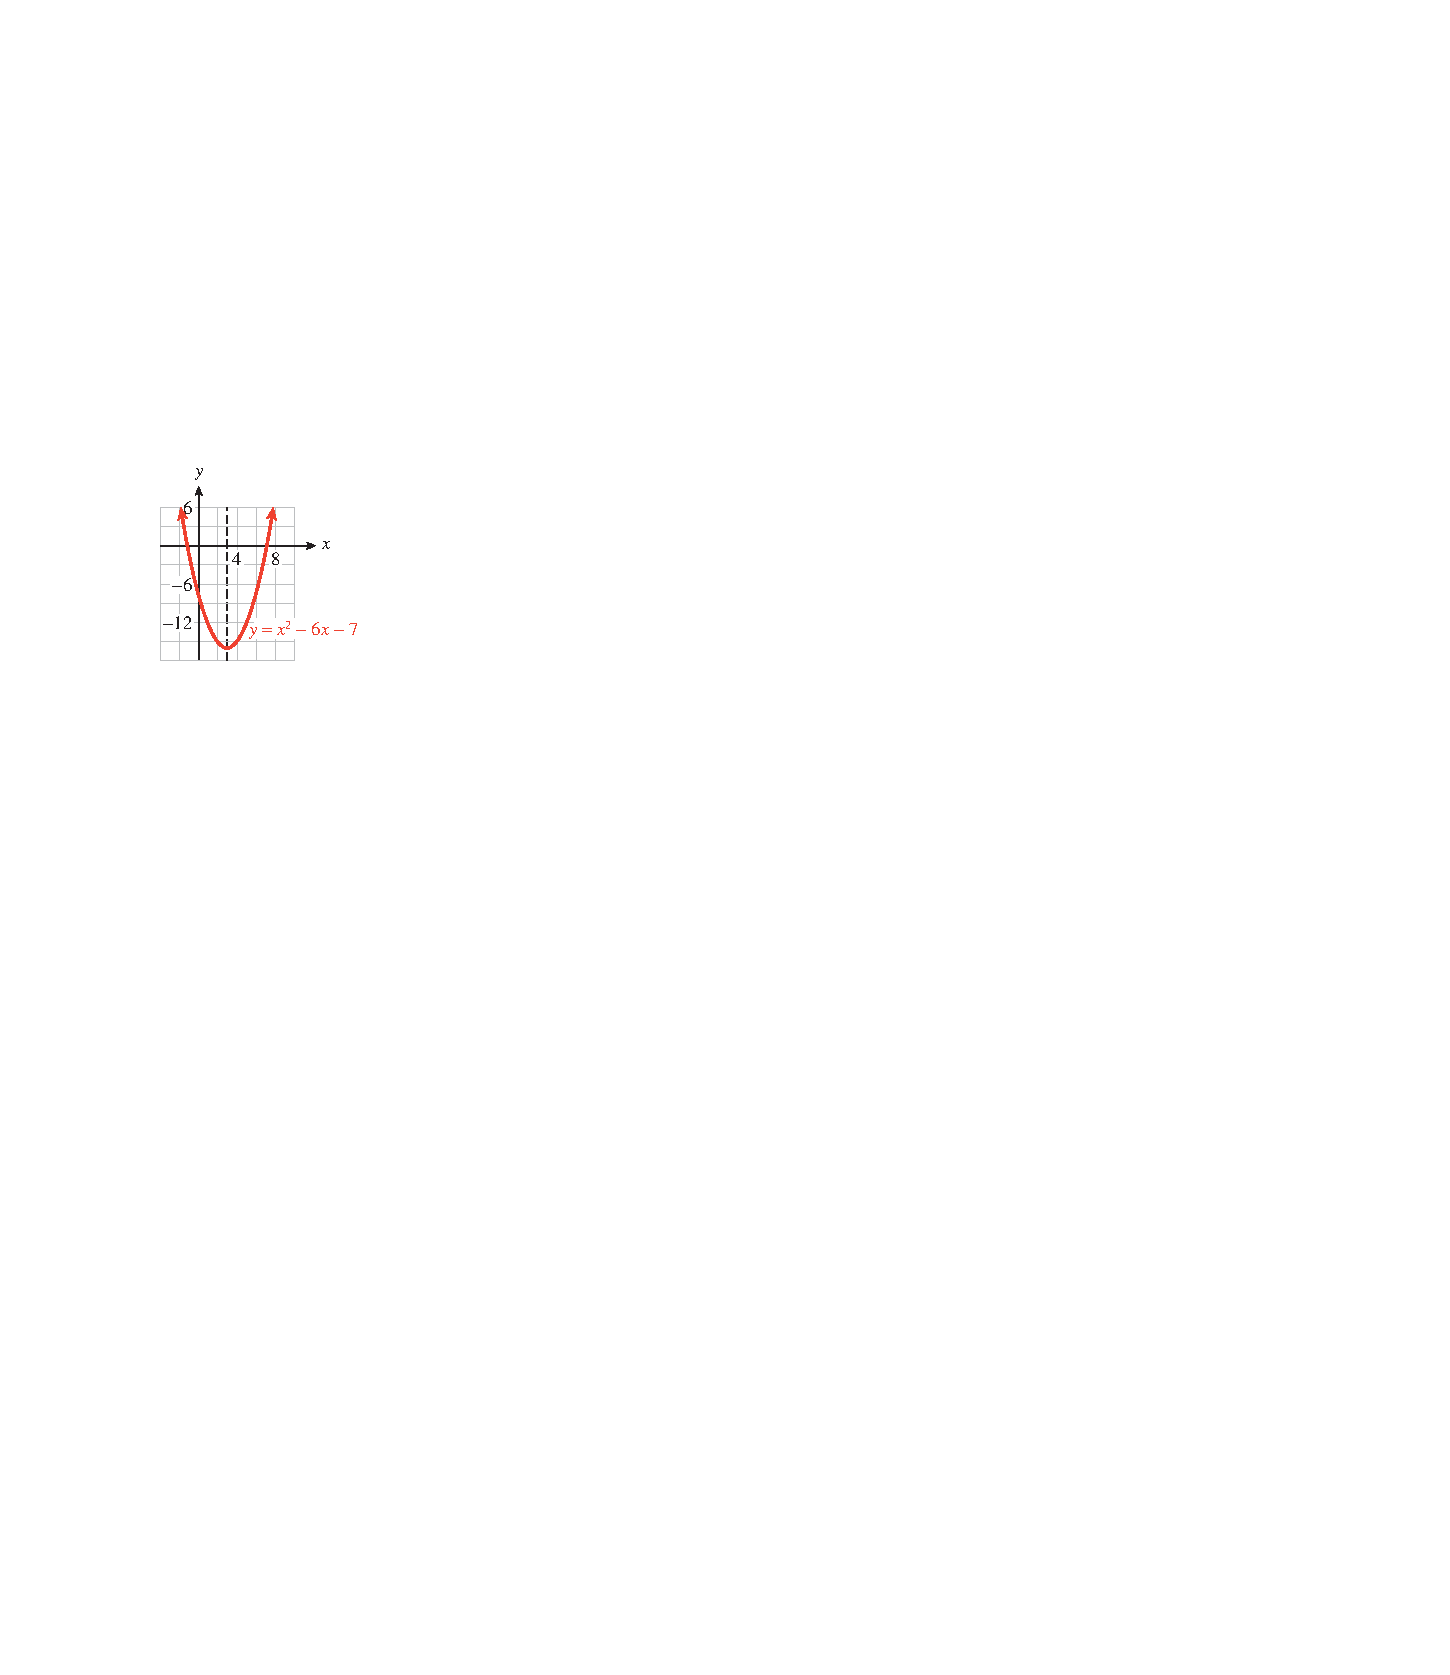
\includegraphics[width=\textwidth,]{images/fig-parabola-with-symmetry-line.pdf}}% end body 
{\captionof{figure}{\label{fig-parabola-with-symmetry-line}}
}% caption 
\pushValignCaptionBottom[c]{minipage}{.70\textwidth}{%
\parbox{\textwidth}{%
% horizontal alignment 

	The graph of \(y = x^2 − 6x − 7\) is shown in \hyperref[fig-parabola-with-symmetry-line]{Figure~\ref{fig-parabola-with-symmetry-line}}. Note that the \(x\)-intercepts of the graph are \(x = 7\) and \(x = −1\), and the parabola is symmetric about the vertical line halfway between the intercepts, at \(x = 3\).
}%
}% end body 
{}% caption 
\popValignCaptionBottom
\end{figure}
\par

	We can also solve \(x^2 − 6x − 7 = 0\) by factoring instead of completing the square. Of course, we get the same solutions by either method. In Example 2, we will solve an equation that cannot be solved by factoring.
%
\begin{example}[]\label{example-completing-the-square2}

		Solve \(x^2 − 4x − 3 = 0\) by completing the square.
	%
\par\medskip\noindent%
\textbf{Solution.}\quad \leavevmode%
\begin{description}
\item[Step 1: ]{}
		Write the equation with the constant term on the right side.
		\begin{equation*}x^2 − 4x{}\text{______}{}=3\end{equation*}\item[Step 2: ]{}
		Now complete the square on the left side. The coefficient of \(x\) is \(−4\), so
		\begin{equation*}p = \frac{1}{2}(−4) = −2 ~~~\text{ and } ~~~ p^2 = (−2)^2 = 4\end{equation*}
		We add \(4\) to both sides of our equation:
		\begin{equation*}x^2 − 4x  \alert{{}+4}=3\alert{{}+4}\end{equation*}\item[Step 3: ]{}
		Write the left side as the square of a binomial, and combine terms on the right side:
		\begin{equation*}(x − 2)^2 =7\end{equation*}\item[Step 4: ]{}
		Finally, use extraction of roots to obtain
		\begin{align*}
		x − 2 \amp =\sqrt{7} \amp\text{or}\amp\amp x − 2 \amp= −\sqrt{7}\amp\text{Solve each equation.}\\
		x \amp =2+\sqrt{7} \amp\text{or}\amp\amp x \amp=2 −\sqrt{7}
		\end{align*}
		The solutions are \(2+\sqrt{7}\approx 4.646\) and \(2−\sqrt{7}\approx −0.646\).
		The graph of \(y = x^2 − 4x − 3\) is shown in \hyperref[fig-parabola-with-symmetry-line2]{Figure~\ref{fig-parabola-with-symmetry-line2}}.
		\leavevmode%
\begin{figure}
\centering
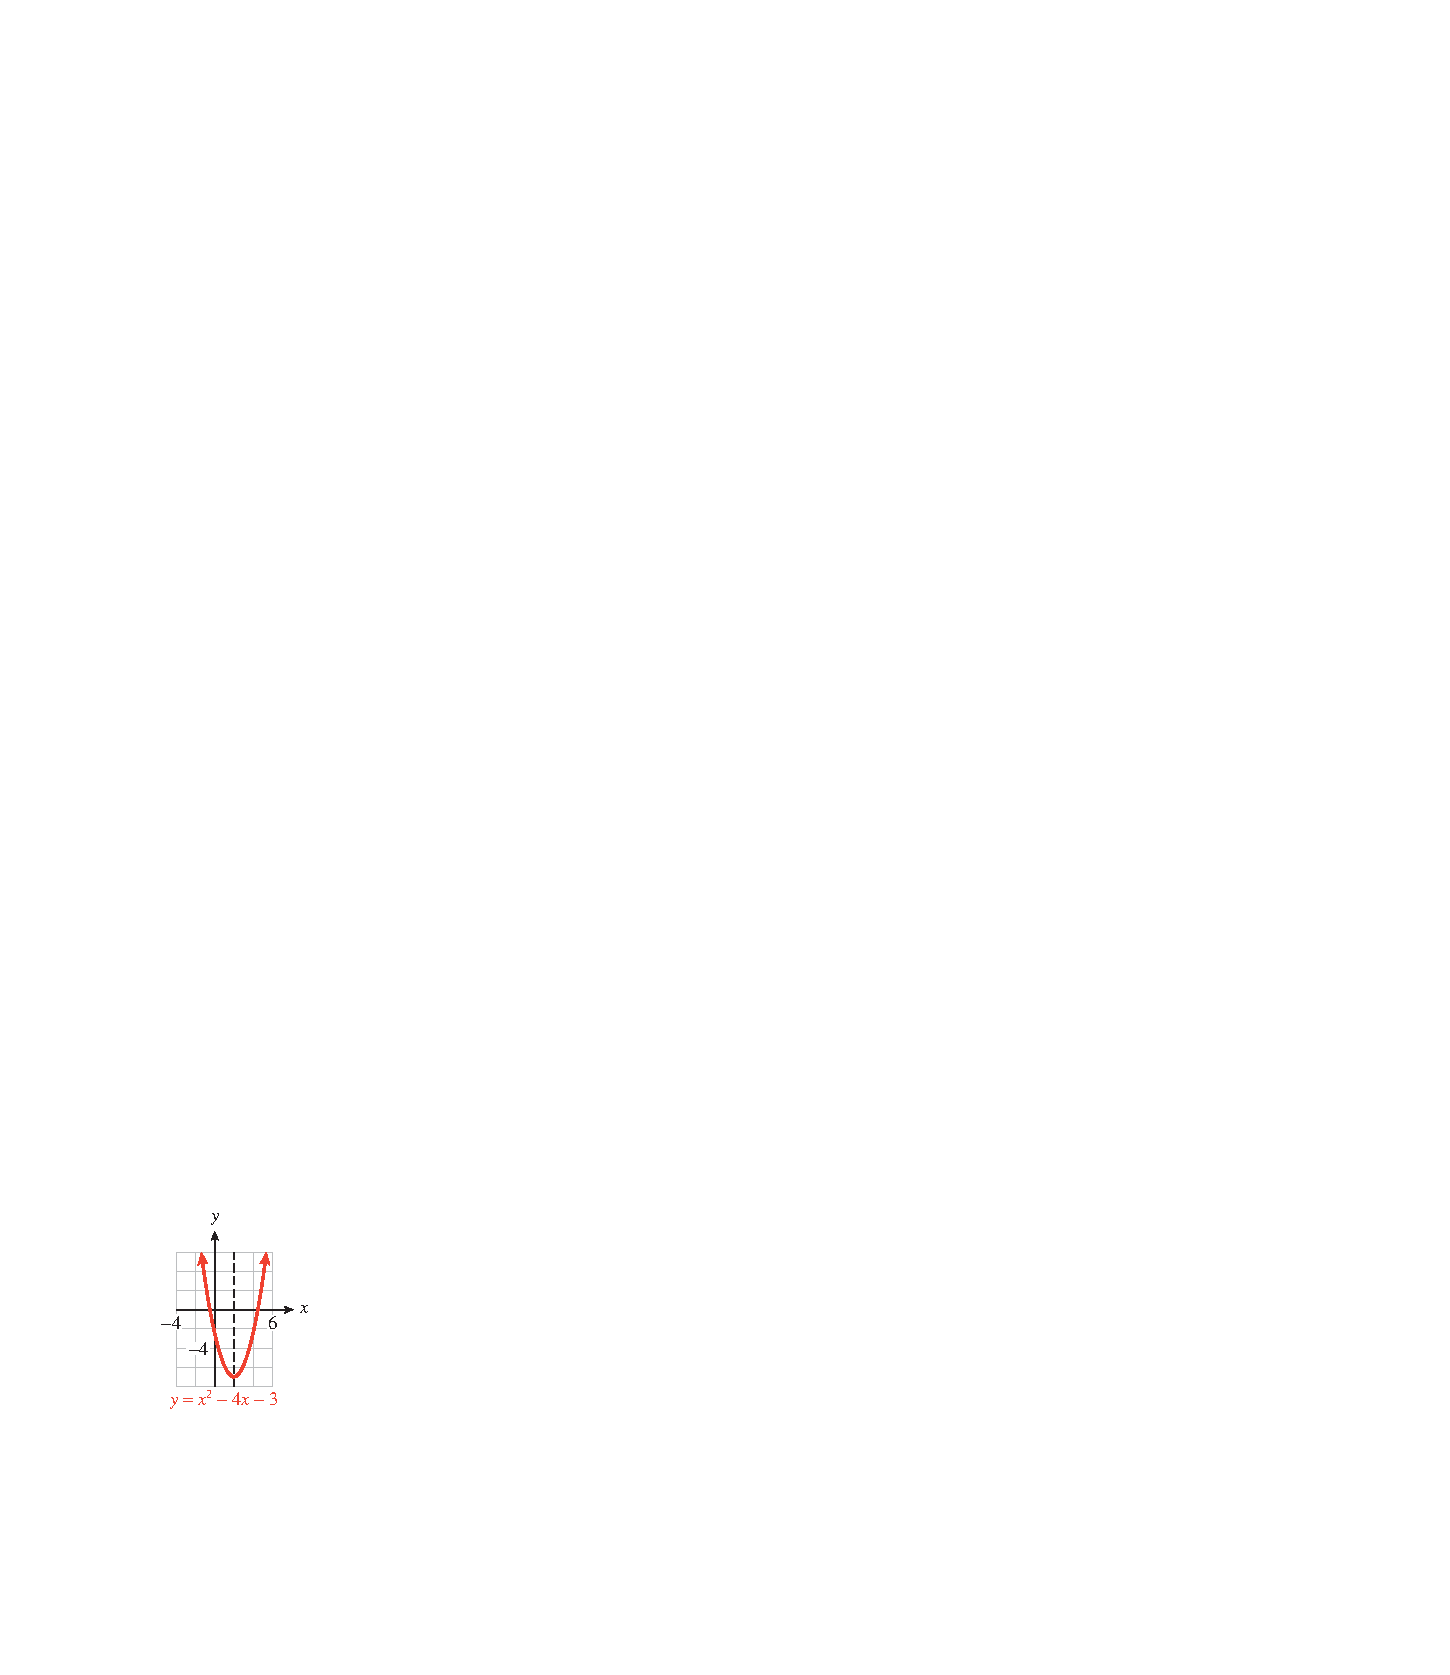
\includegraphics[width=0.45\textwidth,]{images/fig-parabola-with-symmetry-line2.pdf}\caption{\label{fig-parabola-with-symmetry-line2}}
\end{figure}
\end{description}
\end{example}
\begin{exercise}\label{exercise-completing-the-square2}

	\leavevmode%
\begin{enumerate}[label=*\alph**]
\item\hypertarget{li-32}{}
		Follow the steps to solve by completing the square: \(x^2 − 1 = 3x\).
		\begin{description}
\item[Step 1: ]{}
				Write the equation with the constant on the right.
			\item[Step 2: ]{}
				Complete the square on the left:
				\begin{equation*}p = \frac{1}{2}(−3) ={}\text{______, } ~~~{} p^2 = \text{______}\end{equation*}
				Add \(p^2\) to both sides.
			\item[Step 3: ]{}
				Write the left side as a perfect square; simplify the right side.
			\item[Step 4: ]{}
				Solve by extracting roots.
			\end{description}
\item\hypertarget{li-37}{}
		Find approximations to two decimal places for the solutions.
	\item\hypertarget{li-38}{}
		Graph the parabola \(y = x^2 − 3x − 1\) in the window
        \begin{align}
        \text{Xmin} \amp = −4.7 \amp\amp \text{Xmax} = 4.7\\
        \text{Ymin} \amp = −5 \amp\amp \text{Ymax} = 5
        \end{align}
	\end{enumerate}

%
\end{exercise}
\typeout{************************************************}
\typeout{Subsection  The General Case}
\typeout{************************************************}
\subsection[The General Case]{The General Case}\label{subsection-8}

	Our method for completing the square works only if the coefficient of \(x^2\) is \(1\). If we want to solve a quadratic equation whose lead coefficient is not \(1\), we first divide each term of the equation by the lead coefficient.
%
\begin{example}[]\label{example-general-quadratic}

		Solve \(2x^2 − 6x − 5 = 0\).
	%
\par\medskip\noindent%
\textbf{Solution.}\quad \leavevmode%
\begin{description}
\item[Step 1: ]{}
		Because the coefficient of \(x^2\) is \(2\), we must divide each term of the equation by \(2\).
		\begin{equation*}x^2 − 3x − \frac{5}{2}= 0\end{equation*}
		Now we proceed as before. Rewrite the equation with the constant on the right side.
		\begin{equation*}x^2 − 3x \text{______} = \frac{5}{2}\end{equation*}\item[Step 2: ]{}
		Complete the square:
		\begin{equation*}p = \frac{1}{2}(−3) = \frac{-3}{2} ~~~\text{ and } ~~~ p^2 = \left(\frac{-3}{2}\right)^2 = \frac{9}{4}\end{equation*}
		Add \(\frac{9}{4}\) to both sides of our equation:
		\begin{equation*}x^2 − 3x  \alert{{}+\frac{9}{4}}=\frac{5}{2}\alert{{}+\frac{9}{4}}\end{equation*}\item[Step 3: ]{}
		Rewrite the left side as the square of a binomial and simplify the right side to get
		\begin{equation*}\left(x − \frac{3}{2}\right)^2 =\frac{19}{4}\end{equation*}\item[Step 4: ]{}
		Finally, extract roots and solve each equation for \(x\).
		\begin{equation*}
		x − \frac{3}{2}  =\sqrt{\frac{19}{4}} ~~~\text{ or }~~~ x − \frac{3}{2} = −\sqrt{\frac{19}{4}} 
		\end{equation*}
		The solutions are \(\frac{3}{2}+\sqrt{\frac{19}{4}}\) and \(\frac{3}{2}−\sqrt{\frac{19}{4}}\). Using a calculator, we can find decimal approximations for the solutions: \(3.679\) and \(−0.679\).
	\end{description}
\leavevmode%
\begin{enumerate}
\item\hypertarget{li-43}{}
		Because the coefficient of \(x^2\) is \(2\), we must divide each term of the equation by \(2\).
		\begin{equation*}x^2 − 3x − \frac{5}{2}= 0\end{equation*}
		Now we proceed as before. Rewrite the equation with the constant on the right side.
		\begin{equation*}x^2 − 3x \text{______} = \frac{5}{2}\end{equation*}\item\hypertarget{li-44}{}
		Complete the square:
		\begin{equation*}p = \frac{1}{2}(−3) = \frac{-3}{2} ~~~\text{ and } ~~~ p^2 = \left(\frac{-3}{2}\right)^2 = \frac{9}{4}\end{equation*}
		Add \(\frac{9}{4}\) to both sides of our equation:
		\begin{equation*}x^2 − 3x  \alert{{}+\frac{9}{4}}=\frac{5}{2}\alert{{}+\frac{9}{4}}\end{equation*}\item\hypertarget{li-45}{}
		Rewrite the left side as the square of a binomial and simplify the right side to get
		\begin{equation*}\left(x − \frac{3}{2}\right)^2 =\frac{19}{4}\end{equation*}\item\hypertarget{li-46}{}
		Finally, extract roots and solve each equation for \(x\).
		\begin{equation*}
		x − \frac{3}{2}  =\sqrt{\frac{19}{4}} ~~~\text{ or }~~~ x − \frac{3}{2} = −\sqrt{\frac{19}{4}} 
		\end{equation*}
		The solutions are \(\frac{3}{2}+\sqrt{\frac{19}{4}}\) and \(\frac{3}{2}−\sqrt{\frac{19}{4}}\). Using a calculator, we can find decimal approximations for the solutions: \(3.679\) and \(−0.679\).
	\end{enumerate}
\end{example}
\begin{warning}[]\label{warning-1}

		In \hyperref[example-completing-the-square2]{Example~\ref{example-completing-the-square2}}, it is essential that we first divide each term of the equation by \(2\), the coefficient of \(x^2\). The following attempt at a solution is \emph{incorrect}.
		\begin{align*}
		2x^2 − 6x \amp= 5\\
		2x^2 − 6x + 9 \amp= 5 + 9\\
		(2x − 3)^2 \amp= 14 ~~~ \rightarrow ~~~ \text{ Incorrect!}
		\end{align*}
		You can check that \((2x − 3)^2\) is not equal to \(2x^2 − 6x + 9\). We have not written the left side of the equation as a perfect square, so the solutions we obtain by extracting roots will not be correct.
	%
\end{warning}
\end{document}